\documentclass[10pt,a4paper]{article}
\usepackage[utf8]{inputenc}
\usepackage[german]{babel}
\usepackage[T1]{fontenc}
\usepackage{graphicx}
\usepackage{hyperref}
\usepackage{amsmath}
\usepackage{amsfonts}
\usepackage{amssymb}
\usepackage{minted}
\usepackage{wrapfig}
\usepackage{multicol}
\usepackage{vwcol}
\usepackage{tikz}
\usepackage{tikz-qtree}
\usepackage[left=2cm,right=2cm,top=2cm,bottom=2cm]{geometry}
\author{Jonas Betzendahl}
\title{Fortgeschrittene Funktionale Programmiernug in Haskell}

\parindent0pt

\begin{document}

\huge \underline{Fortgeschrittene Funktionale Programmiernug in Haskell}\smallskip

\Large
\begin{center}
\textbf{Projekt:} Entwicklung einer Programmiersprache in Haskell\bigskip

\normalsize
\underline{Tutoren:}
Jonas Betzendahl \texttt{(jbetzend@techfak...)},
Stefan Dresselhaus \texttt{(sdressel@techfak...)}
\end{center}
\normalsize

\section*{\underline{Aufgabenstellung:}}

Ziel dieses Projektes ist die Implementation einer eigenen DSL (\textbf{D}omain \textbf{S}pecific \textbf{L}anguage) zur Erstellung von \href{http://en.wikipedia.org/wiki/Turtle_graphics}{Turtle Grpahics}, ähnlich der Programmiersprache \emph{\textbf{Logo}}.

Hierbei liegt ein Roboter (die \glqq Schildkröte\grqq ) als Cursor in einem 2D-Raum und kann dort umher wandern und geometrische Figuren wie Dreiecke, Spiralen oder Bäume (siehe Bild) zeichnen. 

\subsection*{Mindestanforderungen:}

Ihre Abgabe soll in der Lage sein, eine Datei mit Befehlen für die Schildkröte (s.u.) einzulesen, zu parsen, in eine interne Repräsentation zu überführen und daraus entsprechenden Output zu generieren.\smallskip\smallskip

Sie können mit einer Text-Only Ausgabe beginnen, die nur auf \texttt{stdout} printet, was die Schildkröte tun würde. In der Endabgabe muss allerdings eine grafische Ausgabe generiert werden. Die Wahl der Bibliothek für diese Zwecke (\texttt{sdl2}, \texttt{gtk2hs}, \dots) ist Ihnen frei gestellt.\smallskip\smallskip

\begin{wrapfigure}{R}{0.35\textwidth}
  \vspace{-22pt}
  \begin{center}
    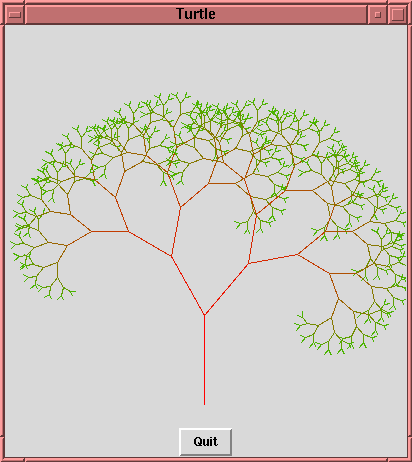
\includegraphics[scale=0.35]{turtle-tree.png} 
  \end{center}
  \vspace{-10pt}
  \caption{Ein möglicher Output der Turtle. Credit: \emph{Chalmers University}}
  \vspace{-40pt}
\end{wrapfigure}

Ihre Programmiersprachen muss zur Abgabe mindestens die folgenden Befehle unterstützen:
\smallskip\smallskip\smallskip

\textbf{forward n}: bewegt die Schildkröte n Einheiten vorwärts\\
\textbf{turn d}: dreht die Schildkröte d Grad im Uhrzeigersinn\\
\textbf{die}: \glqq tötet\grqq\ die Schildkröte (hält das Programm an)\\
\textbf{forever}: führt ein Programm endlos immer wieder aus\\
\textbf{color r g b} oder \textbf{color c}: Verändert die Farbe (Farbwerte oder Name)\\
\textbf{penup/pendown}: hebt/senkt den Stift sodass (nicht) gezeichnet wird
\smallskip\smallskip\smallskip

Sie werden für diese außerdem einen Kombinator wie \texttt{>\%>} implementieren müssen. Dieser führt zwei Programme hintereinander aus. So können sie auch einzelne Befehle zu
komplexeren Programmen zusammenfügen. Welche der oben aufgeführten Befehle lassen sich auf eine Kombination
von simpleren Befehlen zurück führen?

\subsection*{Zusatz:}

Bei besonderer Motivation können außerdem die folgenden Features noch eingebaut werden:\bigskip
 
\begin{minipage}{0.68\linewidth}
\begin{itemize}
\item \textbf{Parallel Turtles:}\\ Implementieren sie den Operator \texttt{<\%>} analog zu \texttt{>\%>}. Dieser startet beide Programme parallel (es gibt also danach eine zusätzliche Schildkröte).
\item \textbf{Schildkröten-Funktionen:}\\ Geben Sie Ihrer Programmiersprache die Möglichkeit, Funktionen auszudrücken (z.B. analog zum Code rechts), die dann ebenfalls als Programme aufgerufen werden können.
\end{itemize}
\end{minipage}
\hfill
\begin{minipage}{0.3\linewidth}
\begin{verbatim}
 Schildkröten-Funktion:
 
 to spiral :size :angle
   if :size > 100 [stop]
   forward :size
   right :angle
   spiral :size + 2 :angle
 end
\end{verbatim}
\end{minipage}

\section*{\underline{Abgabemodalitäten:}}

Eine gültige Abgabe ist ein \texttt{cabal}-Projekt, das fehlerfrei in einer Sandbox installiert werden kann und eine funktionierende ausführbare Datei generiert (Testumgebung ist im Zweifelsfall wie immer das GZI). Bitte reichen Sie Ihre Projekte spätestens bis zum \textbf{Freitag, den 18.09.2015} ein.
Dazu schicken Sie alle Dateien, die zu Ihrem Projekt gehören (eventuell modulo einer vernünftigen \texttt{.gitignore}) in einem Dateiarchiv an beide Tutoren.\bigskip

Falls gewünscht, kann Ihnen für die Entwicklung des Projekts ein privates Repository auf \texttt{GitHub} zur Verfügung gestellt werden. Dann kann auch direkt dort abgegeben werden. Kontaktieren Sie dafür bitte die Tutoren.\bigskip

Sollten Sie Rückfragen haben oder Hilfestellung benötigen, wenden Sie sich bitte ebenfalls an die Tutoren.

\end{document}